\documentclass{beamer}
\usetheme{Pittsburgh}
\beamertemplatenavigationsymbolsempty


\usepackage{amsmath}
\usepackage{amssymb}
\usepackage{bm} % For bold math symbols
\usepackage{graphicx}
\usepackage{tikz}



\usepackage{subfig} % Changed from subfigure (deprecated)
\usepackage{multirow}
\usepackage{multicol}
\usepackage{color}
\usepackage{url}
\usepackage{hyperref}
\usepackage{listings}
\usepackage[noend]{algorithm}
\usepackage{physics} 
% add image path
\graphicspath{{../Images/}}






\DeclareMathOperator{\argmin}{argmin}
\DeclareMathOperator{\argmax}{argmax}






\title{Weekly Updates\\
\tiny{Tuesday, 04/03/2025}}
\author{Andrea Bonifacio}
\date{}

\begin{document}

\begin{frame}
\titlepage
\end{frame}


\begin{frame}{Neural Modes Paper - Key Ideas}
    \begin{itemize}
        \item The paper wants to extend the concept of linear modes to ``neural modes''.
        \item The idea is to compute a non-linear correction of the displacement field, by having the network minimize the energy of the system.
        \item Once the network has been trained and learned the non-linear modes for any modal coordinate in the subspace, it can be extended to dynamics by using a finite difference scheme.
    \end{itemize}
\end{frame}



\begin{frame}
\frametitle{My implementation}
\begin{itemize}
    \item Computed eigenmodes by solving the generalized eigenvalue problem: \( K \mathbf{v} = \lambda M \mathbf{v} \)
    \begin{itemize}
        \item \( K \) is the stiffness matrix.
        \item \( M \) is the mass matrix.
        \item \( \mathbf{v} \) are the eigenvectors (modes).
        \item \( \lambda \) are the eigenvalues (squared frequencies).
    \end{itemize}
    \item After computing the \(n\) modes, create the \(m\) dimensional subspace by selecting the first \(m\) modes.
    \begin{itemize}
        \item How to select the modes?
        \item How to enforce boundary conditions?
    \end{itemize}
\end{itemize}
\end{frame}

\begin{frame}
    \frametitle{Some modes}

    \begin{figure}
        \centering
        \includegraphics[width=0.45\textwidth]{Images/mode_9.png}
        \includegraphics[width=0.45\textwidth]{Images/mode_10.png}
        \caption{Two eigenmodes of the mesh.}
        \label{fig:eigenmodes}
    \end{figure}
\end{frame}

\begin{frame}
    \frametitle{Network Architecture}
    \begin{itemize}
        \item The network is a feedforward neural network.
        \item The input is the modal coordinate \( z \in \mathbb{R}^m \).
        \item The output is a correction on the displacement field \( \mathbf{y} \in \mathbb{R}^n \).
    \end{itemize}



\begin{center}
        
        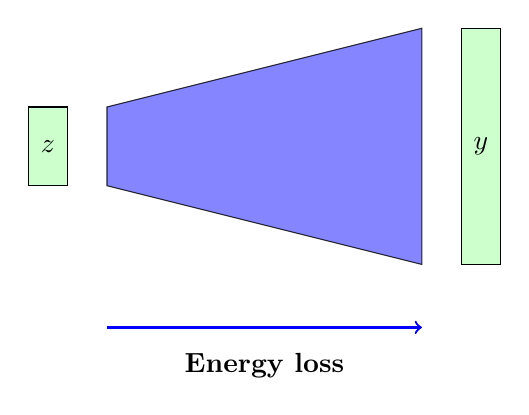
\begin{tikzpicture}
            % Modal coordinate (z)
            \draw[fill=green!20] (-3, 1) rectangle (-2.5,2);
            \node at (-2.75, 1.5) {$z$}; % Label inside the rectangle
            
            % Displacement (u)
            \draw[fill=green!20] (2.5,0) rectangle (3,3);
            \node at (2.75, 1.5) {$y$}; % Label inside the rectangle
            
            % Energy loss transition
            \draw[fill=blue!60,opacity=0.8] (-2,1) -- (2,-0) -- (2,3) -- (-2,2) -- cycle;
            \node[below] at (0,-1) {\textbf{Energy loss}};
            
            % Energy loss arrow
            \draw[thick,blue,->] (-2,-0.8) -- (2,-0.8);
        
        \end{tikzpicture}
\end{center}
    
\end{frame}

\begin{frame}
    \frametitle{Training the network}
    \begin{itemize}
        \item At each iteration, the network is trained on a batch of modal coordinates randomly selected.
        \item Three loss functions are used:
        \begin{itemize}
            \item Energy loss: \( E(X + l + y)\), where \(X\) is the rest position, \(l\) is the linear mode given by \(z\) and \(y\) is the nonlinear correction.
            \item Orthogonality loss: \( y^T l = 0 \).
            \item Origin loss: \( y(0) = 0 \).
        \end{itemize}
        \item The network is trained by minimizing the sum of the three losses.
        \[
        \text{Loss} = \text{Energy } + \lambda_1 \text{Orthogonality } + \lambda_2 \text{Origin}
        \]
    \end{itemize}
\end{frame}

\begin{frame}
    \frametitle{Dynamic simulation}
    I haven't implemented this part yet, but the core idea is to use the trained network to compute the non-linear correction at each time step.
    \begin{itemize}
        \item Given the finite difference scheme:
        \[
          u_{n+1} = \underset{u}{\argmin}  \frac{1}{2h^2} \norm{u - 2u_n + u_{n-1}}^2_M + E(u)
        \]
        \item The non-linear correction can be computed by:
        \[
        z_{n+1} = \underset{z}{\argmin}  \frac{1}{2h^2} \norm{n(z) - 2u_n + u_{n-1}}^2_M + E(n(z))
        \]
        \item Here \(n(z)\) is the non-linear correction computed by the network, and \(M\) is the mass matrix.
    \end{itemize}
\end{frame}

\begin{frame}
    \frametitle{Next steps}
    \begin{itemize}
        \item Implement a SOFA compatible version of the code.
        \item Implement the dynamic simulation.
        \item Learn how to do simulations correctly
    
    \end{itemize}
\end{frame}

% Q&A
\begin{frame}
    \begin{center}
        \Huge{Questions?}
    \end{center}

\end{frame}
\end{document}

